\chapter{The Finite Element Method}
\section{Boundary value problems}
In this section we will define a general initial boundary value problem (I-BVP). In the first part we will introduce the differential formulation given in terms of a set of governing equations and properly specified boundary conditions. The resulting equations are obtained after using a generalized balance law. Following this classical and well known approach we will introduce the variational formulation where the governing equations and natural boundary conditions are now obtained after solution of an extremization problem of a so-called functional. It will become evident that the resulting extremization problem is equivalent to the weak form of the problem defined previously.
%%
\subsection{Differential formulation}
Let $ds$ be a differential surface element; $dV$ a differential volume element; $u(\vec x,t)$ a scalar (or vector) function of space and time.
The flux or rate of flow of the quantity $u(\vec x,t)$ through $ds$ at time $t$ is defined like;
\[p(\vec x)\vec \nabla u \cdot \hat nds\]

where $p(\vec x)$ is a positive function, assumed known and time independent. Similarly, the time rate of change of $u(\vec x,t)$ in an element $dV$ is given by;

\[\rho (\vec x)\frac{{\partial u}}{{\partial t}}dV\]

where once again $\rho (\vec x)$ is a known, given, time independent positive function. Additional effects occurring in the element $dV$ at the time time can be expressed like;

\[H(\vec x,t)dV \equiv  - q(\vec x)u(\vec x,t) + \hat F(\vec x,t)\]

where $\hat F(\vec x,t) = \rho (\vec x)F(\vec x,t)$. In the above the term $qu$ represent internal effects due to changes proportional to $u$ while $\hat F(\vec x,t)$ are other external inlfuences in the medium.

Balancing the internal and external changes yields;

\[\int\limits_V {\rho (\vec x)\frac{{\partial u}}{{\partial t}}dV = \int\limits_S {p(\vec x)\vec \nabla u \cdot \hat nds} }  + \int\limits_V {H(\vec x,t)dV} \]

or equivalently;

\[\int\limits_V {\rho (\vec x)\frac{{\partial u}}{{\partial t}}dV = \int\limits_S {p(\vec x)\vec \nabla u \cdot \hat nds} }  - \int\limits_V {q(\vec x)u(\vec x,t)dV}  + \int\limits_V {\rho (\vec x)F(\vec x,t)dV} \]

using the divergence theorem as

\[\int\limits_S {p(\vec x)\vec \nabla u \cdot \hat nds}  = \int\limits_V {\vec \nabla  \cdot \left( {p\vec \nabla u} \right)dV} \]

yields after substitution;

\[\int\limits_V {\left[ {\rho (\vec x)\frac{{\partial u}}{{\partial t}} - \vec \nabla  \cdot \left( {p(\vec x)\vec \nabla u} \right) + q(\vec x)u(\vec x,t) - \rho (\vec x)F(\vec x,t)} \right]dV}  = 0\]

Assuming a continuous integrand, the arbitrariness of $V$ implies;

\[
\rho (\vec x)\frac{{\partial u}}{{\partial t}} - \vec \nabla  \cdot \left( {p(\vec x)\vec \nabla u} \right) + q(\vec x)u(\vec x,t) - \rho (\vec x)F(\vec x,t) = 0
\]

Letting;

\[L() \equiv  - \vec \nabla  \cdot \left( {p(\vec x)\vec \nabla } \right) + q(\vec x)\]

the generalized set of partial differential equations can be written like;

\begin{equation}
\rho (\vec x)\frac{{\partial u(\vec x,t)}}{{\partial t}} + Lu(\vec x,t) = \rho (\vec x)F(\vec x,t)
\label{GenPDE}
\end{equation}

Hyperbolic;
\[\rho (\vec x)\frac{{{\partial ^2}u(\vec x,t)}}{{\partial {t^2}}} + Lu(\vec x,t) = 0\]
Parabolic;
\[\rho (\vec x)\frac{{\partial u(\vec x,t)}}{{\partial t}} + Lu(\vec x,t) = 0\]
Elliptic;
\[Lu(\vec x,t) = \rho (\vec x)F(\vec x,t)\]
\section{Brief review of the linearized theory of elasticity model}
Here we present a brief description of the boundary value problem governing the response of an elastic body. For a full discussion of the model and its mathematical aspects the reader is referred to \cite{shames1997elastic}.

The governing equations (in terms of stresses) stem from the principle of conservation of linear momentum and conservation of moment of linear momentum. The former leads to a set of 3 partial differential equations in the components of the stress tensor while the latter leads to the symmetries in the stress tensor.

\begin{equation} \label{eq:pde}
\begin{aligned}
&\sigma_{ij,j} + {f_i} = \rho\ddot{u}_i \quad \forall\ \vb{x} \in V,\, t \in \mathbb{R}^{+}\\
&\sigma_{ij}=\sigma _{ji}.
\end{aligned} 
\end{equation}

In \cref{eq:pde} $\sigma_{ij}$ is the stress tensor; $f_i$ is the vector of body forces; and $u_i$ is the displacements vector.

Denoting the tractions vector associated with a surface with normal direction $\hat{n}_{j}$ by $t_i^{\hat n}$ we have the complete BVP as follows:

\begin{equation} \label{eq:bcs}
t_i^{\hat n} = \sigma_{ij} \hat{n}_{j} \quad \forall \in \vb{x} \in S.
\end{equation}

\Cref{eq:pde} correspond to 6 equations with 12 unknowns (the 9 components of the stress tensor and the 3 components of the displacements vector ) and the system is undetermined. In order to have a solvable BVP we must introduce kinematic strain-displacement relations and a stress-strain law. In the case of infinitesimal theory of elasticity the strain-displacement relation is given by:

\begin{equation}\label{eq:kin}
\varepsilon_{ij} = \frac{1}{2}(u_{i,j} + u_{j,i})
\end{equation}

where the term $\epsilon_{ij}$ is the symmetric component of the displacements gradient tensor. The components of the strain tensor describe the distrotions and changes in magnitude (volumetric changes) of the material point in the continuum model. Now the simplest stress-strain (constituive) relationship is given by Hooke's law\footnote{Despite the name of \emph{law} used, this relation is not always valid, but is a good approximation for small strains.}

\begin{equation} \label{eq:Hooke}
\sigma_{ij} = 2\mu \varepsilon_{ij} + \lambda \varepsilon_{kk}\delta_{ij} \enspace .
\end{equation}

where $\mu$ and $\lambda$ are material constants. The problem involves now a total of 18 equations and 18 unknowns can be solved if subjected to properly specified boudnary conditions.

\subsection*{Displacement formulation}
Substituting \cref{eq:kin} in \cref{eq:Hooke} and the result in \cref{eq:pde} yields after some manipulation:

\begin{equation} \label{eq:navier}
(\lambda  + \mu)u_{j,ij} + \mu u_{i,jj} + {f_i} = \rho \ddot{u}_i \quad \forall \vb{x} \in V,\, t \in \mathbb{R}^{+}.
\end{equation}

Since \cref{eq:navier} ( simultaneously describing equilibrium, kinematic relations and constituive response) is a second order equation governing the displacemt field possible boundary conditions are in terms of the variable itself or its first oder derivatives. For a well-possed problem the following is a set of valid boundary conditions: 

\begin{equation} \label{eq:Wellbcs}
\begin{split}
&t_i^{\hat n} = \sigma _{ij} \hat n_{ij} \quad \forall\ \vb{x} \in S_t\\
& {u_i} = \bar{u}_i \quad \forall \vb x \in S_u
\end{split}
\end{equation}

and where ${S_t} \cup {S_u} = S$ and ${S_t} \cap {S_u} = \emptyset $. 


In the particular case in which $u_i$ is not a function of time, we obtain the static version of the BVP, i.e,
\begin{equation}
\begin{split}
&\left(\lambda  + \mu \right)u_{j,ij} + \mu u_{i,jj} + {f_i} = 0 \quad \forall \vb{x} \in V \\
&t_i^{\hat n} = \sigma _{ij} \hat n_{ij} \quad \forall\ \vb{x} \in S_t\\
& {u_i} = \bar{u}_i \quad \forall \vb x \in S_u
\end{split}
\end{equation}

Notice that the tractions BC 
\[t_i^{\hat n} = \mu (u_{i,j} + u_{j,i}) \hat{n}_j + \lambda u_{k,k} \delta_{ij}\hat{n}_j \enspace ,\]

actually involves first order displacemts derivative and as such it is a Neumann boundary condition on $u_i$.
%

\subsection{Equivalence between strong and weak forms}
\subsubsection{Strong form}
The strong form corresponds to the differential formulation of the problem, it is denoted by $\{ S \}$ and it reads:

Given $f_i$, $t_i^{\hat n}$ and ${\bar u_i}$ find ${u_i}:V \to \mathbb{R}$ such:
%
\begin{equation} \label{eq:navier_2}
\begin{split}
&(\lambda  + \mu)u_{j,ij} + \mu u_{i,jj} + f_i = 0 \quad \forall \vb{x} \in V \\
&t_i^{\hat n} = \sigma _{ij} \hat{n}_{ij} \quad \forall \vb{x} \in S_t\\
&u_i = \bar{u}_i \quad \forall \vb{x} \in S_u
\end{split}
\end{equation}

In \cref{eq:navier_2} the boundary conditions specified by the traction vector $t_i^{\hat n}$ correspond to the natural boundary conditions, while those specified in terms of the displacements vector $\bar u_i$ represent the essential boundary conditions.

\begin{itemize}
\item We are interested in developing methods to obtain approximate solutions to $\{S\}$.
\item The FEM is formulated starting from a statement equivalent to $\{ S \}$ in which we use trial functions until certain prescribed conditions are met.
\item We will look for solutions $u_i$ subject to the following conditions:
\begin{align*}
&u_i = \bar u_i\\
&\intL_S \left(\pdv{u_i}{x_j} \right)^2 dS < \infty
\end{align*}

\end{itemize}

The first condition corresponds to the satisfaction of the essential boundary condition, while the second corresponds to the functions being square integrable. The space of functions satisfying the above two conditions is denoted by $\varsigma$ and formally defined like
%
\[\varsigma = \left\{u_i\left| {u_i} \in H, {u_i} = \bar{u}_i \in S_u \right. \right\} \enspace .\]
%
On the other hand, in order to validate the introduced trial functions we also need testing functions $w_i$ also called in the FEM literature weighting or distribution functions. These functions are arbitrary apart from having to satisfy the following conditions:
%
\begin{align*}
&w_i = 0 \quad in \quad {S_u}\\
&\intL_S \left(\pdv{w_i}{x_j}\right)^2 dS < \infty
\end{align*}
%
In what follows we formally denote the space of these functions by $V$ and define it like
%
\[V = \left\{ w_i\left| w_i \in H, u_i = w_i=0 \in S_u \right. \right\} \enspace .\]

\subsubsection{Weak form}
Here we will show that the equilibrium statement represented in the differential formultaionthe problem can be described in an alternative forms. In such description the continuity requirement for the trial functions is weaker than in the strong form leading to the term "weak" statement. Here this alternative representation will be denoted like $\{W\}$ and it reads;

Given $f_i$, $t_i^{\hat n}$ and ${\bar u_i}$ find ${u_i}:V \to \mathbb{R}$ and $\forall {w_i} \in V$ such:

\[\intL_V \sigma _{ij,j} w_{i,j}\, dV - \intL_V f_i w_i\, dV  - \intL_{S_t} t_i^{\hat n} w_i\, dS = 0\]

\subsubsection*{Proof 1:}
Let $u_i \in \varsigma $ be a solution to $\{S\}$ and let $w_i \in V $. Forming the inner product of the equilibrium statement given in \cref{eq:pde} with $w_i$ and forcing the integral over the domain to be zero we have
%
\[\intL_V (\sigma_{ij,j} + f_i ){w_i}\, dV = 0 \enspace ,\]
%
expanding the terms in the integrand and integrating by parts the first term on the left we have
%
\[\intL_V \sigma _{ij,j} w_i\, dV + \intL_V f_i w_i\, dV = 0 \enspace .\]
\[ - \intL_V w_{i,j} \sigma _{ij}\, dV  + \intL_S \sigma _{ij} \hat{n}_j w_i\, dS  + \intL\limits_V w_i f_i\, dV = 0 \]

since $w_i \in V$ it follows that $w_i = 0$ in $S_u$ from which

\begin{equation}\label{weak}
\intL_V \sigma _{ij,j} w_{i,j}\, dV - \intL_V f_i w_i\, dV  - \intL_{S_t} t_i^{\hat n} w_i\, dS = 0
\end{equation}

Now, considering that $u_i$ is solution of the strong form $\{S\}$ it must satisfy $u_i = \bar u_{i} \quad \in \quad S_u$ and as a result $u_i \in \varsigma$. On the other hand, since $u_i$ satisfies \cref{weak} $\forall {w_i} \in V$ we have that $u_i$ satisfies the definition of weak solution specified in $\{ W \}$.

\subsubsection*{Proof 2:}
Let $u_i$ be a solution of $\{W\}$ and thus $u_i \in \varsigma$ which means that
\[u_i = \bar u_{i} \quad \in \quad S_u\]
and that it satisfies
\[\intL_V \sigma _{ij} w_{i,j}\, dV - \intL_V f_i w_i\, dV - \intL_{S_t} t_i^n w_i\, dS = 0 \enspace ,\]
integrating by parts,
\[-\intL_V \sigma_{ij,j} w_idV + \intL_S \sigma_{ij} n_j w_i dS  - \intL_V f_i w_i dV - \intL_{S_t} {t_i^n} w_i dS = 0\]

Since ${w_i} \in V$ we have that ${w_i}=0$ in $S_u$ and therefore
\[\intL_V w_i(\sigma_{ij,j} + f_i)dV + \intL_{S_t} w_i( \sigma_{ij} n_j - t_i^n )dS = 0 \]
from which
\begin{equation} \label{equil_2}
\begin{split}
&\sigma_{ij,j} + f_i = 0 \quad \vb{x} \in V \\
&t_i^n = \sigma_{ij} n_j \quad \forall \vb{x} \in S_t\\
&{u_i} = \bar{u}_i \quad \forall \vb{x} \in S_u
\end{split}
\end{equation}

which is once again the strong form of the problem given in \cref{eq:pde}.

\subsection*{Simple wedge under self-equilibrated loads}
Consider the double wedge of side $\ell$ and internal angle $2 \phi$ shown in \cref{fig:WEDGE}. It is assumed to be contained in the $X-Y$ plane, with loading conditions satisfying a plane strain (or plane stress) idealization. The material is elastic with Lame constants $\lambda$ and $\mu$. The wedge is loaded by uniform tractions of intensity $S$ applied over its four faces in such a way that the wedge is self-equilibrated. We wish to find the closed-form elasticity solution for the stress, strain and displacement fields throughout the problem domain.
%
\begin{figure}[H]
\centering
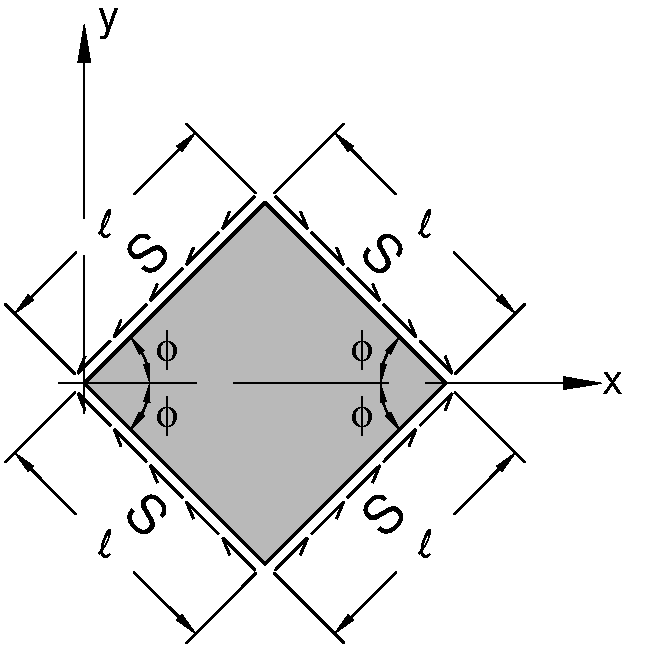
\includegraphics[width=7cm]{img_src/wedge.pdf}
\caption{2D Self-equilibrated wedge.}
\label{fig:WEDGE}
\end{figure}

Under plane strain conditions the general 3D stress equilibrium equations (see \cref{eq:pde}) reduce to:
\begin{equation}
\begin{aligned}
&\pdv{\sigma_{xx}}{x}+\pdv{\tau_{xy}}{y}=0\\
&\pdv{\tau_{xy}}{x}+\pdv{\sigma_{yy}}{y}=0
\end{aligned}
\label{eq:equilibrium}
\end{equation}

while the kinematic relation (\cref{eq:kin}) reads

\begin{equation}
\begin{aligned}
\epsilon_{xx}&=\pdv{u}{x}\\
\epsilon_{yy}&=\pdv{v}{y}\\
\gamma_{xy}&=\pdv{u}{y} + \pdv{v}{x}
\end{aligned}
\label{eq:strain}
\end{equation}
where $u$ and $v$ are the horizontal and vertical displacements respectively.

\subsubsection*{Stress field}

The stress field can be obtained by simple inspection from the traction boundary conditions prescribed over the inclined surfaces yielding;

\begin{align*}
\sum F_x &= 0 \longrightarrow - \ell S\cos(\phi)  + \sigma_{xx}\ell \sin(\phi) = 0\\
\sum F_y &= 0 \longrightarrow - \ell S\sin(\phi) - \sigma_{yy}\ell \cos(\phi)=0
\end{align*}

and the following stress solution:

\begin{equation}
\begin{aligned}
\sigma_{xx}& = S \cot(\phi)\\
\sigma_{xx}& = -S\tan(\phi)\\
\tau_{xy}& = 0.
\end{aligned}
\label{eq:solution}
\end{equation}

In \cref{eq:solution} the condition $\tau_{xy}=0$ is due to symmetrie in the problem.

\subsubsection*{Traction boundary conditions}
Let us verify that the above stress solution satisfies the traction BC using the expression:

\[t_i^{\hat n} = \sigma _{ij} \hat n_{ij}.\]

Donoting the outward normals to the inclined surfaces of the wedge by $\hat{n}^1$,  $\hat{n}^2$, $\hat{n}^3$, $\hat{n}^4$ these are given by;
\begin{align*}
\hat{n}^1 &= -\sin(\phi)\hat{e}_{x}+\cos(\phi)\hat{e}_{y}\\
\hat{n}^2 &= -\sin(\phi)\hat{e}_{x}-\cos(\phi)\hat{e}_{y}\\
\hat{n}^3 &= +\sin(\phi)\hat{e}_{x}+\cos(\phi)\hat{e}_{y}\\
\hat{n}^4 &= +\sin(\phi)\hat{e}_{x}-\cos(\phi)\hat{e}_{y} \enspace
\end{align*}

where $\hat{e}_{x}$ and $\hat{e}_{y}$ are the reference unit vectors. Now, the components of the traction vector follow directly like

\[t_{i} = \sigma_{ij}\hat{n}_{j}\]

then over the face with normal $\hat{n}^1$ we have
\begin{align*}
t_{x} &= -S\cos(\phi)\\
t_{y} &= -S\sin(\phi)
\end{align*}
similarly, over the face with normal $\hat{n}^2$
\begin{align*}
t_{x} &= -S\cos(\phi)\\
t_{y} &= +S\sin(\phi)
\end{align*}
over the face with normal $\hat{n}^3$ 
\begin{align*}
t_{x} &= +S\cos(\phi)\\
t_{y} &= -S\sin(\phi)
\end{align*}
and finally, over the face with normal $\hat{n}^4$;
\begin{align*}
t_{x} &= +S\cos(\phi)\\
t_{y} &= +S\sin(\phi) \enspace .
\end{align*}

\subsubsection*{Strain field}
The strain field can be obtained after using the stress solution found in \cref{eq:solution} together with the constituive law given by \cref{eq:Hooke} which for a plane strain idalization takes the form:

\begin{equation}
\begin{aligned}
\epsilon_{xx}& = +\dfrac{S}{E}\left[\cot(\phi)+\nu \tan(\phi)\right] = +\dfrac{S}{E}K_{1}(\nu , \phi)\\
\epsilon_{yy}& = -\dfrac{S}{E}\left[\tan(\phi)+\nu \cot(\phi)\right] = -\dfrac{S}{E}K_{2}(\nu , \phi)\\
\gamma_{xy}& = 0.
\end{aligned}
\label{eq:strain part}
\end{equation}

\subsubsection*{Displacement field}
The displacement field is obtained after direct integration of the strains after using the fact that:

\[du_i=\epsilon_{ij}dx_j + \omega_{ij}dx_j\]

and the condition $\omega_{xy}=0$ also due to symmetrie , as follows:

\begin{align*}
u &= +\dfrac{S}{E} K_{1}(\nu , \phi)x + A\\
v &= -\dfrac{S}{E} K_{2}(\nu , \phi)y + B
\end{align*}

and where $A$ and $B$ are integration constants.

From the condition $u=0$ at $x=\ell\cos(\phi)$ we have that $A=-\dfrac{S}{E} K_{1}(\nu , \phi)\ell\cos(\phi)$ then it follows that
\[u=\dfrac{S}{E} K_{1}(\nu , \phi)(x-\ell\cos(\phi)).\]

Similarly, from the condition $v=0$ at $y=0$ we have that $B=0$ from which
\[v=-\dfrac{S}{E} K_{2}(\nu , \phi)y\]



%%
\subsection{Variational formulation}
In this section we formulate the boundary value problem using the approach of the calculus of variations in which the governing PDEs and boundary conditions are obtained after finding the minimum (or maximum) of a functional according to a variational principle\footnote{According to Wikipedia \cite{wiki:variational_principle}

\begin{quotation}
A variational principle is a scientific principle used within the calculus of variations, which develops general methods for finding functions which minimize or maximize the value of quantities that depend upon those functions. For example, to answer this question: ``What is the shape of a chain suspended at both ends?" we can use the variational principle that the shape must minimize the gravitational potential energy.

According to Cornelius Lanczos, any physical law which can be expressed as a variational principle describes an expression which is self-adjoint. These expressions are also called Hermitian. Such an expression describes an invariant under a Hermitian transformation.
\end{quotation}}.
%%
We will see that the weak form (and therfore also the strong form) can be obtained alternatively through the process of finding extreme values for a functional. We will ilustrate this idea for the general case of theory of elasticity and then we will present particular examples.

\subsubsection*{Some vague definitions in the calculus of variations}
In variational calculus a {\bf functional} can be understood as a "function" having as independent variables or arguments a space of vector functions and producing as a result (or dependent variable) a scalar. For instance, in the particular case of the theory of elasticity such a "function" corresponds to the total potenatial energy functional $\Pi$ given by;

\begin{equation}
\Pi ({u_i}) = \frac{1}{2}\int\limits_V {{\sigma _{ij}}{\varepsilon _{ij}}dV}  - \int\limits_V {{f_i}{u_i}dV}  - \int\limits_S {t_i^{(n)}{u_i}dS}
\label{Potential}
\end{equation}

and where the first term in the L.H.S corresponds to the internal strain energy, while the last two terms are the work done by the external body and traction forces. The above functional has as independent variables the displacement vector and its spatial derivatives. This is indicated by the presence of the displacement vector $u_i$ in the expression $\Pi(u_i)$.

In variational calculus we are interested in finding a function $u_i$ that renders the functional $\Pi$ a maximum or a minimum. In loose terms, the analogous to the differential operator in calculus of functions is now termed the variational operator $\delta$ (i.e., $\delta$ is analogous to $\frac{\partial }{{\partial {x_i}}}$). As such $\delta\Pi$ acts over the function $u_i$ and its derivatives as follows;

\[\delta \Pi  = \frac{{\partial \Pi }}{{\partial {u_i}}}\delta {u_i} + \frac{{\partial \Pi }}{{\partial \left( {\frac{{\partial {u_i}}}{{\partial {x_j}}}} \right)}}\delta \left( {\frac{{\partial {u_i}}}{{\partial {x_j}}}} \right) + ... + \frac{{\partial \Pi }}{{\partial \left( {\frac{{{\partial ^n}{u_i}}}{{\partial {x_j}...\partial {x_k}}}} \right)}}\delta \left( {\frac{{{\partial ^n}{u_i}}}{{\partial {x_j}...\partial {x_k}}}} \right)\].

The following rules apply to the variational operator $\delta$:

\begin{itemize}
\item For functionals $\Pi$ and $\Phi$ it follows that \[\delta (\Pi  + \Phi ) = \delta \Pi  + \delta \Phi \]
\item For functionals $\Pi$ and $\Phi$ it follows that \[\delta (\Pi \Phi ) = \delta \Pi \Phi  + \Pi \delta \Phi \]
\item For a functional $\Pi$ and an integer $n$ it follows that \[\delta ({\Pi ^n}) = n({\Pi ^{n - 1}})\delta \Pi \]
\item For a functional $\Pi$ it follows that \[\delta \int {\Pi dx}  = \int {\delta \Pi dx} \]
\end{itemize}

If the variational operator is applied to the functional $\Pi (u_i)$ it produces functions or variations in $u_i$ which are arbitrary and such $\delta {u_i} \in V$ and $\delta {u_i} = 0$ in $S_u$.

In order to find an extreme function in the calculus of variations we proceed like in differential calculus. Here we compute the first variation of the functional $\delta \Pi$ and solve the variational equation;

\begin{equation}
\delta \Pi  = 0
\label{vareq}
\end{equation}

in the unknown function $u_i$. 

In the particular case of the total potential energy functional $\Pi$ this yields;

\begin{equation}
\int\limits_V {{\sigma _{ij}}\delta {\varepsilon _{ij}}dV}  - \int\limits_V {{f_i}\delta {u_i}dV}  - \int\limits_{{S_t}} {t_i^{(n)}\delta {u_i}dS}  = 0
\label{ClaPVW}
\end{equation}

where we recognize the weak form of the BVP stated previously. It becomes evident that the functions $\delta {u_i}$ in \cref{ClaPVW} play the role of the test functions $w_i$ introduced in the weak form. On the other hand, since we have already shown that the weak and strong forms are equivalent we conclude that having the functional and the escential boundary conditions is equivalent to having the strong form of the problem.


\subsubsection*{Principle of minimum potential energy}
In the theory of elasticity the total potential energy $\Pi$ is the result of adding the elastic strain energy which is stored in the body upon deformation and the potential energy (work) imparted to the body by the applied forces. The principle states that the body is in equilibrium when this total potential energy reaches a minimum. This is equivalent to stating that an equilibrium configuration is attained when an infinitesimal variation from the position of minimum potential energy involves null changes in energy. This implies the variational condition:

\begin{equation}
\delta \Pi  = 0.
\label{vareq2}
\end{equation}

The above principle leads to the so-called principle of virtual displacements stated as follows\footnote{see Bathe pp 156}:
"The equlibrium of the body requires that for any compatible small virtual displacements satisfying the condition of being zero at $S_u$, imposed on the body in its state of equilibrium, the total internal virtual work is equal to the total external virtual work"

\[\int\limits_V {{\sigma _{ij}}\delta {\varepsilon _{ij}}dV}  - \int\limits_V {{f_i}\delta {u_i}dV}  - \int\limits_{{S_t}} {t_i^{(n)}\delta {u_i}dS}  = 0\]

where ${\delta {u_i}}$ are the virtual displacements and ${\delta {\varepsilon _{ij}}}$ are the corresponding virtual strains.

Comparing the virtual work principle with the weak formulation given in \cref{weak} we identify ${\delta {u_i}}$ with the test functions $w_i$. As such the PVW takes the form of a powerful tool to test if a body is in equilibrium for a given solution (represented by the trial functions). In what follows we ilustrate the use of the principle through some examples corresponding to problems in Bathe's textbook.

\subsubsection*{Problem 3.15}\todo{add the figure corresponding to this problem}
Establish the differential equation of equilibrium of the problem shown and the boundary conditions. Determine whether the differential operator of the problem is symmetric and positive definite and prove your answer.

\[\Pi  = \frac{1}{2}\int\limits_0^L {{\sigma _{xx}}{\varepsilon _{xx}}A(x)dx} + \frac{1}{2}ku_0^2 - R{u_L} \]
\[\Pi  = \frac{1}{2}\int\limits_0^L {EA(x){{\left( {\frac{{du}}{{dx}}} \right)}^2}dx + \frac{1}{2}ku_0^2}  - R{u_L}\]

First variation;
\[\delta \Pi  = \int\limits_0^L {EA(x)\frac{{du}}{{dx}}\frac{{d\delta u}}{{dx}}dx + k{u_0}\delta {u_0}}  - R\delta {u_L}\]

Integrating by parts;

\[\delta \Pi  =  - \int\limits_0^L {\frac{d}{{dx}}\left[ {EA(x)\frac{{du}}{{dx}}} \right]\delta udx + \left. {EA(x)\frac{{du}}{{dx}}\delta u} \right]_0^L + k{u_0}\delta {u_0}}  - R\delta {u_L}\]

from which;

\[\frac{d}{{dx}}\left[ {EA(x)\frac{{du}}{{dx}}} \right] = 0\]
\[{\left. {EA(x)\frac{{du}}{{dx}}} \right]_{x = 0}} = k{u_0}\]
\[{\left. {EA(x)\frac{{du}}{{dx}}} \right]_{x = L}} = R\]





\subsubsection*{Problem 4.35-The Hu-Washizu Variational Principle}
Consider the Hu-Washizu functional:
\begin{equation}
\Pi^* = \Pi  - \intL_V \lambda_{ij}^\varepsilon (\varepsilon_{ij} - L_{ijk} u_k)\dd{V}  - \intL_{S_u} \lambda_i^u(u_i^{S_u} - \bar{ u}_i)\dd{S}
\label{eq:Hu}
\end{equation}

where
\begin{itemize}
\item $\Pi$: is the potential energy functional.
\item $L_{ijk}$ is a differential operator such $\varepsilon_{ij} = L_{ijk} u_k$.
\item $S_u$ surface where essential boundary conditions are prescribed.
\item $\lambda_{ij}^\varepsilon $ and $\lambda_i^u$ are Lagrange multipliers.
\end{itemize}

Using the condition $\delta \Pi = 0$ derive for the interior of the body the equlibrium equations;

\[{\sigma _{ij,j}} + {f_i} = 0\]

the strain-displacement relationship;

\[{\varepsilon _{ij}} = {L_{ijk}}{u_k}\]

and the constitutive equation;

\[{\sigma _{ij}} = {C_{ijkl}}{\varepsilon _{kl}}\]

and at the surface of the body the relation between the stress tensor and the applied tractions vector at $S_t$;

\[{t_i} = {\sigma _{ij}}{n_j}\]

the relation between the stress tensor and the unknown tractions vector (or reactions) at $S_u$; 

\[{t_i} = {{\tilde \sigma }_{ij}}{n_j}\]

and the escential boundary condition at $S_u$;

\[{u_i} = {{\tilde u}_i}\]

We want to determine the so-called Euler equations resulting from the condition $\delta \pi^* = 0$. Applying the variational operator we have:
\begin{equation}
\begin{aligned}
\delta \Pi^*& = \delta \Pi  - \intL_V \delta \lambda_{ij}^{\varepsilon}  (\varepsilon_{ij} - L_{ijk} u_k)\dd{V}- \intL_V \lambda_{ij}^\varepsilon (\delta \varepsilon_{ij} - L_{ijk}\delta u_k)\dd{V} \\
&-\intL_V \delta \lambda_i^u (u_i^{S_u} - \bar u_i)\dd{S} - \intL_V \lambda _i^u \delta u_i^{S_u} \dd{S}
\end{aligned}
\end{equation}

\begin{equation}
\begin{aligned}
\delta \Pi^* &= \intL_V C_{ijkl} \varepsilon_{kl} \delta  \varepsilon_{ij}\dd{V} - \intL_{S_t} t_i \delta{u_i} \dd{S}  - \intL_V f_i\delta {u_i}\dd{V} - \intL_V \lambda_{ij}^{\varepsilon} \delta \varepsilon_{ij}\dd{V}  + \intL_V \lambda_{ij}^{\varepsilon} L_{ijk}\delta {u_k}\dd{V}\\
&- \intL_V \delta \lambda_{ij}^{\varepsilon} (\varepsilon_{ij} - L_{ijk} u_k)\dd{V} - \intL_S \delta \lambda_i^u (u_i^{S_u} - \bar {u}_i)dS - \intL_{S_u} \lambda _i^u\delta {u_i}\dd{S} = 0
\end{aligned}
\end{equation}

using

\[\intL_V {(\lambda _{ij}^\varepsilon \delta {u_i}){,_j}dV = } \intL_V {\lambda _{ij}^\varepsilon \delta {u_{i,j}}dV}  + \intL_V {\lambda _{ij,j}^\varepsilon \delta {u_i}dV} \]

in the above we can write

\begin{align*}
\intL_V {\lambda _{ij}^\varepsilon {L_{ijk}}\delta {u_k}dV} & = \intL_V {{{(\lambda _{ij}^\varepsilon \delta {u_i})}_{,j}}dV}  - \intL_V {\lambda _{ij,j}^\varepsilon \delta {u_i}dV}\\
& = \intL_{{S_t}} {\lambda _{ij}^\varepsilon \delta {u_i}{{\hat n}_j}dS}  - \intL_V {\lambda _{ij,j}^\varepsilon \delta {u_i}dV}
\end{align*}

therefore


\begin{align*}
\delta \Pi^* &= \intL_V {({C_{ijkl}}{\varepsilon _{kl}} - \lambda _{ij}^\varepsilon )\delta {\varepsilon _{ij}}dV - \intL_{{S_t}} {{t_i}\delta {u_i}dS}  - \intL_V {{f_i}\delta {u_i}dV + } } \intL_{{S_t}} {\lambda _{ij}^\varepsilon \delta {u_i}{{\hat n}_j}dS}  - \intL_V {\lambda _{ij,j}^\varepsilon \delta {u_i}dV}\\
&- \intL_V {\delta \lambda _{ij}^\varepsilon ({\varepsilon _{ij}} - {L_{ijk}}{u_k})dV}  - \intL_{{S_u}} {\delta \lambda _i^u(u_i^{{S_u}} - {{\bar u}_i})dS}  - \intL_{{S_u}} {\lambda _i^u\delta {u_i}dS}  = 0
\end{align*}


\begin{align*}
&\intL_V {({C_{ijkl}}{\varepsilon _{kl}} - \lambda _{ij}^\varepsilon )\delta {\varepsilon _{ij}}dV
+ \intL_{{S_t}} {(\lambda _{ij}^\varepsilon {{\hat n}_j} - {t_i})\delta {u_i}dS}  - }\\
&\intL_V {(\lambda _{ij,j}^\varepsilon  + {f_i})\delta {u_i}dV}
- \intL_V {({\varepsilon _{ij}} - {L_{ijk}}{u_k})\delta \lambda _{ij}^\varepsilon dV}
- \intL_{{S_u}} {(u_i^{{S_u}} - {{\bar u}_i})\delta \lambda _i^udS}  - \cancel{\intL_{{S_u}} {\lambda _i^u\delta u_i^{{S_u}}dS} = } 0
\end{align*}


Now, imposing the conditions $\delta {\varepsilon _{ij}} \neq 0$, $\delta \lambda _{ij}^\varepsilon  \neq 0$, $\delta {u_i} \neq 0$ in $S_t$, $\delta {u_i} \neq 0$ in $V$ and $\delta \lambda _i^u \neq 0$ in $S_u$ we have
%
\begin{align}
&\lambda _{ij}^\varepsilon  = C_{ijkl} \varepsilon_{kl}\\
&\varepsilon_{ij} = {L_{ijk}}{u_k}\\
t_i &= \lambda_{ij}^\varepsilon \hat{n}_j\\
&\lambda _{ij,j}^\varepsilon  + {f_i} = 0\\
&u_i^{S_u} = \bar{u}_i
\end{align}

\subsection{Weighted residual methods}
In the the following derivations we will assume that the actual solution to the geberalized BVP is approximated by the superposition;

\[u(\vec x) = {N^I}(\vec x){u^I}\]

where $I=1,2,...,K$.

Since we are now using an approximation we have the following "unbalanced" condition;

\[Lu(\vec x,t) - \rho (\vec x)F(\vec x,t) = R \ne 0\]

where the term $R$ corresponds to a residual error which is to be distributted trhoughout the solution domain.



\subsubsection*{Application to the Navier equations}

\[(\lambda  + \mu ){u_{j,ij}} + \mu {u_{i,jj}} + {f_i} = 0\]
\[{L_{ij}} \equiv (\lambda  + \mu )\frac{{{\partial ^2}}}{{\partial {x_i}\partial {x_j}}} + \mu \frac{{{\partial ^2}}}{{\partial {x_k}\partial {x_k}}}{\delta _{ij}}\]
\[{r_i} =  - {f_i}\]
\[{u_i} = N_i^Q{u^Q}\]
\[{L_{ij}}({u_j}) \equiv (\lambda  + \mu ){(N_j^Q{u^Q})_{,ij}} + \mu {(N_j^Q{u^Q})_{,kk}}{\delta _{ij}}\]
\[{L_{ij}}({u_j}) \equiv (\lambda  + \mu )N_{j,ij}^Q{u^Q} + \mu N_{i,kk}^Q{u^Q}\]
\[{L_{ij}}({u_j}) \equiv {L_{ij}}(N_j^Q){u^Q}\]

In the Galerkin scheme we use the trial function as weigthing function.

\[{R_i} \equiv {L_{ij}}(N_j^Q){u^Q} + {f_i}\]

and we state



\subsubsection*{Application to the acoustic wave equation}

\section[Discretization of the PVW using FEM]{Discretization of the PVW via the FEM}
\subsection*{A simple spring-mass system}
The simple problem of a spring-mass system considered next resembles most of the algorithmic aspects of a finite element code with the advantage that the problem is already a discrete mechanical system. The problem consists of an assamblage of masses joined by different springs submitted to time varying loads. Each spring plays the role of a finite element and each mass is analogous to a nodal point in a finite element algorithm. For instance the full system may be like the one shown in \cref{fig:bathe}:


\begin{figure}[H]
\centering
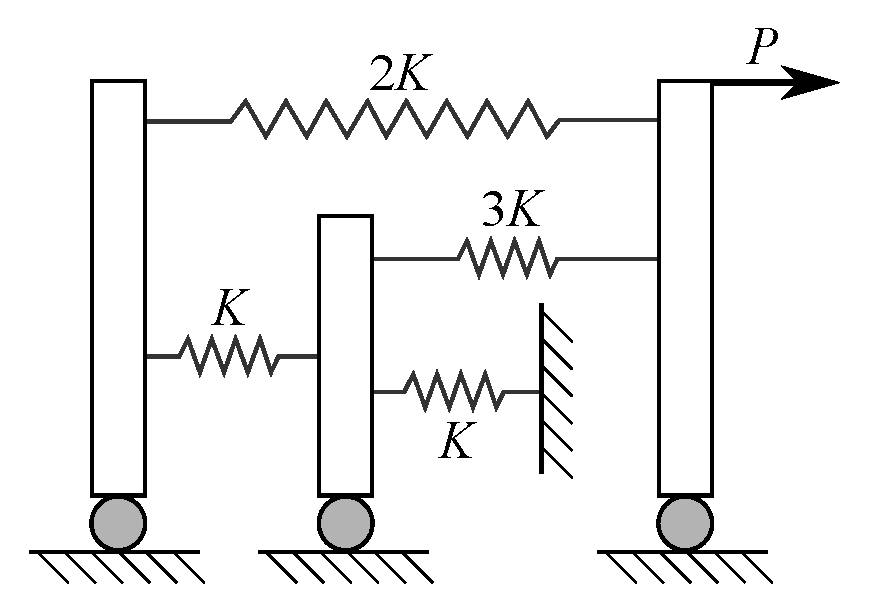
\includegraphics[width=10cm]{img/spring_system.pdf}
\caption{Typical assemblage of springs and masses.}
\label{fig:bathe}
\end{figure}


Consider a typical spring (finite element) like the one shown in \cref{fig:springel}

\begin{figure}[H]
\centering
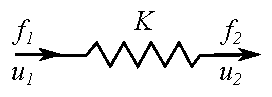
\includegraphics[width=10cm]{img/springel.pdf}
\caption{Typical spring element.}
\label{fig:springel}
\end{figure}

The relation between the force and the relative displacement can be written like;

\[{f_1} = K({u_1} - {u_2})\]

and from equilibrium we have;

\[{f_1} + {f_2} = 0\]

which yields the following force-displacement relationship for a tyical spring element:

\begin{equation}
\left\{ {\begin{array}{*{20}{c}}
{{f_1}}\\
{{f_2}}
\end{array}} \right\} = K\left[ {\begin{array}{*{20}{c}}
{1.0}&{ - 1.0}\\
{ - 1.0}&{1.0}
\end{array}} \right]\left\{ {\begin{array}{*{20}{c}}
{{u_1}}\\
{{u_2}}
\end{array}} \right\}
\label{Kspring}
\end{equation}

On the other hand, the equilibrium equation for a typical mass with displacement $u_j$  (see \cref{fig:dclmass}) and attached to springs $i$ and $i+1$ read;

\begin{equation}
f_2^i + f_1^{i + 1} + {m_j}\frac{{d{V_j}}}{{dt}} = {P_j}.
\label{equilmass}
\end{equation}

which can be written in terms of displacements using \cref{Kspring} like;

\[({K^i} + {K^{i + 1}}){u_j} - {K^i}{u_{j - 1}} - {K^{i + 1}}{u_{j + 1}} + {m_j}\frac{{d{V_j}}}{{dt}} = {P_j}.\]


\begin{figure}[H]
\centering
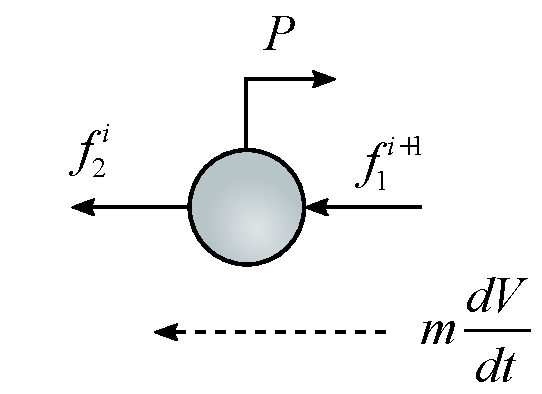
\includegraphics[width=8cm]{img/dcl_mass.pdf}
\caption{Free body diagram for a typical mass connceted to springs $i$ and $i+1$.}
\label{fig:dclmass}
\end{figure}

Considering now the complete system of masses and springs leads to a system of linear equations of the form;

\begin{equation}
\left[ {{K_G}} \right]\left\{ {{U_G}} \right\} + \left[ M \right]\left\{ {{A_G}} \right\} = \left\{ {{F_G}} \right\}.
\label{global}
\end{equation}

where each equation represents the equilibrium of a given mass. The system given by \cref{global} can be solved in the displacements $U_G$. The pseudo-code shown in \cref{springsalg} presents all the steps required to sove the problem in the context of the finite element method. In that code the so-called DME operator is an equation assembly array indicating how each element contributes to the global stiffness and mass matrix.


\begin{algorithm}[H]
 \SetAlgoLined
 \KwData{Problem paramters; NUMNP, NUMEL, NMATP}
 \KwResult{Displacements and spring forces}
 Create $DM$E operator\;
 Assemble $K^G$, $F^G$\;
\While{$j \leq 1, NUMEL$}{
\[
\begin{aligned}
K^G \leftarrow K^G+K^i\\
F^G \leftarrow F^G+F^i\\
\end{aligned}
\]
}
Impose BCs\;
Solve $[K^G]U=F^G$\\
Find internal forces
\caption{Springs Algorithm}
\label{springsalg}
\end{algorithm}


\subsection{Basic elements of interpolation theory}
Let $f(x)$ be a function whose values are known at n discrete points ${x_1, x_2,...,x_n}$. We want to know (interpolate) the value of $f(x)$ at an arbitrary point $x \in \left[ {{x_1},{x_n}} \right]$.

\begin{figure}[h]
\centering
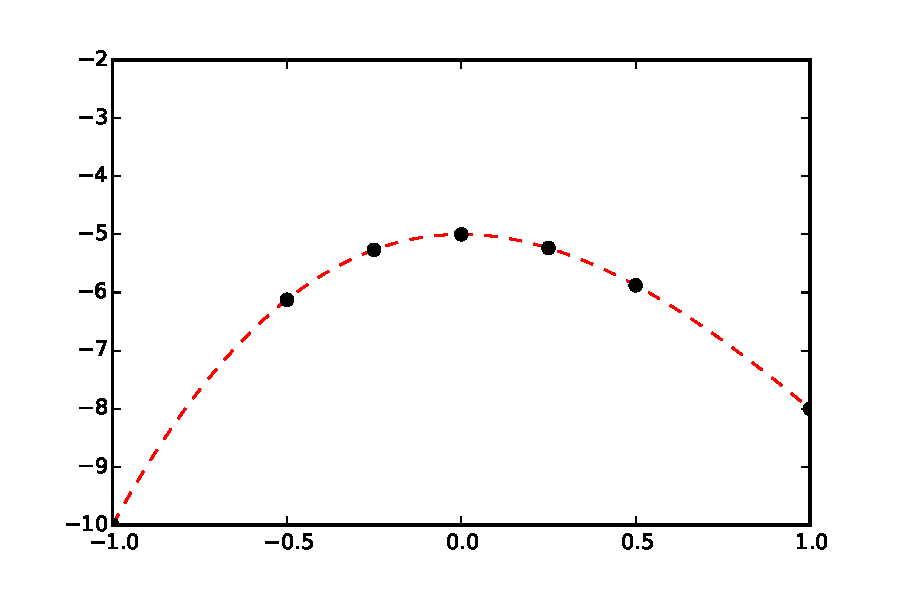
\includegraphics[width=8cm]{img/interpol1.pdf}
\caption{Definition of the natural domain}
\label{fig:interpol1}
\end{figure}

The process of interpolation or computation of the unknown value of $f(x)$ using the known values $\left\{ {{f^1},{f^2},...,{f^n}} \right\}$ involves two steps:

\begin{itemize}
\item[i]  Fitting an interpolating function to the known data points.
\item[ii] Evaluating the function at the arbitrary point.
\end{itemize}

We can (i) use all the n-data points and fit an $(n-1)$-th order polynomial (which is cumbersome and difficult to code) or (ii) split the domain in sub-intervals and use local polynomials within each sub-interval. This last approach involves only a couple of polynomials and it is easy to code, however it may have some continuity issues.

In finite element analysis local interpolation is used in order to proceed systematically. Local interpolation uses a finite number of nearest-neighbours and generates interpolated values $f(x)$ that do not in general have continuous first or higher derivatives.

\begin{figure}[h]
\centering
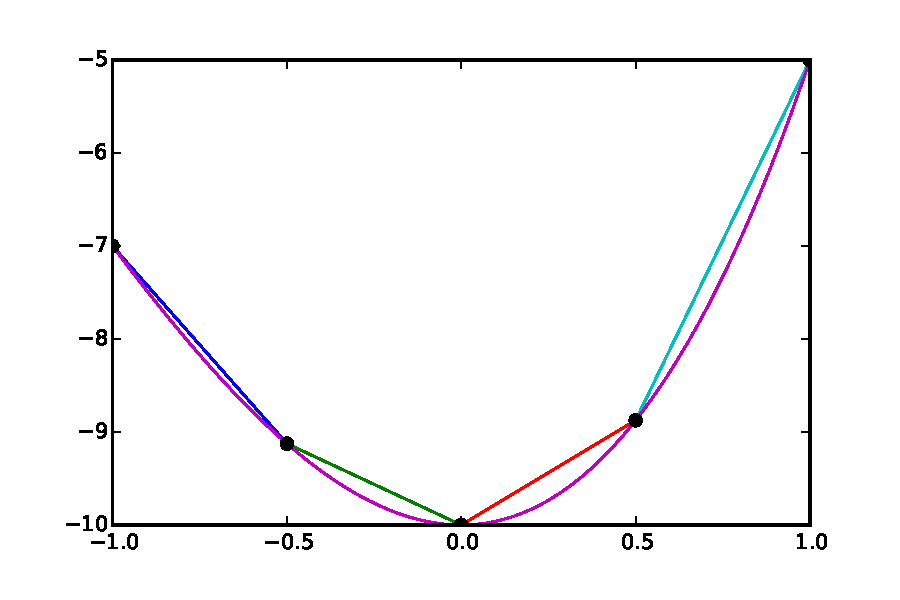
\includegraphics[width=8cm]{img/interpol2.pdf}
\caption{Definition of the natural domain}
\label{fig:interpol2}
\end{figure}

\subsubsection{Lagrange interpolation theorem}
Given a set of n-points $\left\{ {({x^1},{y^1}),...,({x^n},{y^n})} \right\}$ where ${y^n} \equiv f({x^n})$ then: "there exists a unique polynomial $p(x)$ of order at most $(n-1)$ such $p({x^I}) = f({x^I})$ for $I=1,2,...,n$". The polynomial is given by;

\begin{equation}
p({x^I}) = {L^I}(x)f({x^I})
\label{pol}
\end{equation}

for $I=1,2,...,n$ where;

\begin{equation}
{L^I}(x) = \prod\limits_{\scriptstyle J = 1\hfill\atop
\scriptstyle I \ne J\hfill}^n {\frac{{(x - {x^J})}}{{({x^I} - {x^J})}}}
\label{coef}
\end{equation}

and where it should be noticed that

\[{L^I}({x^J}) = {\delta ^{IJ}}.\]

\subsubsection*{Example for n=3}

Consider the domain $[ - 1,1]$ and the data points at ${x^1} =  - 1.0$, ${x^2} =  + 1.0$ and ${x^3} = 0.0$. We have
\[{L^1}(x) = \frac{{\left( {x - {x^2}} \right)\left( {x - {x^3}} \right)}}{{\left( {{x^1} - {x^2}} \right)\left( {{x^1} - {x^3}} \right)}} \equiv  - \frac{1}{2}\left( {1 - x} \right)x\]
\[{L^2}(x) = \frac{{\left( {x - {x^1}} \right)\left( {x - {x^3}} \right)}}{{\left( {{x^2} - {x^1}} \right)\left( {{x^2} - {x^3}} \right)}} \equiv  + \frac{1}{2}\left( {1 + x} \right)x\]
and
\[{L^3}(x) = \frac{{\left( {x - {x^1}} \right)\left( {x - {x^2}} \right)}}{{\left( {{x^3} - {x^1}} \right)\left( {{x^3} - {x^2}} \right)}} \equiv 1 - {x^2}.\]

The resulting interpolating polynomials ${L^I}(x)$ and the interpolating function  are shown in \cref{fig:pols} below:

\begin{figure}[H]
\centering
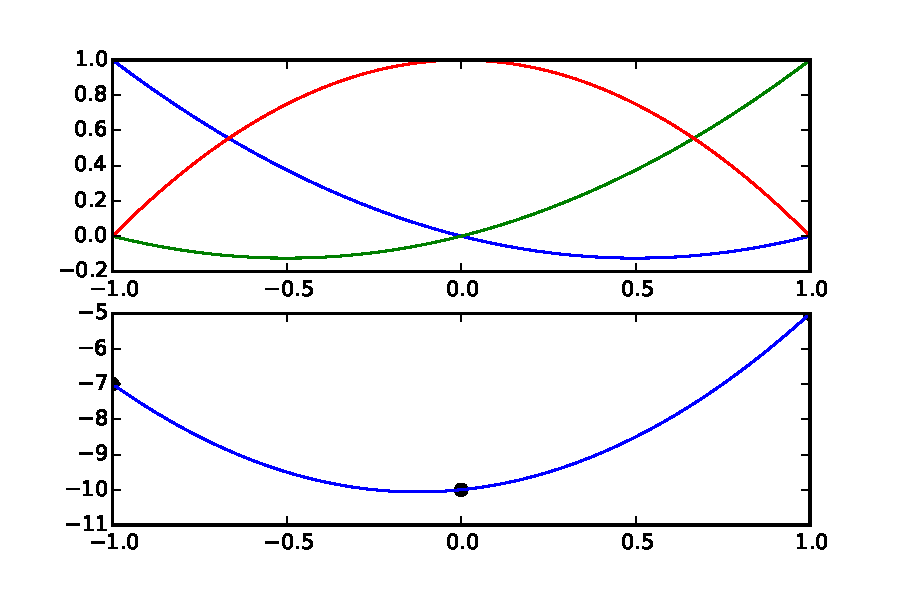
\includegraphics[width=16cm]{img/func.pdf}
\caption{Interpolating polynomials and the resulting interpolating function}
\label{fig:pols}
\end{figure}

\subsection*{Extension to 2D domains}
Assume we are now interested in conducting interpolation of a function over a spatial 2-dimensional domain where every point is specified by a position vector of the form $\vec x = x\hat i + y\hat j$. We want to know, via interpolation, the value of a function $f(\vec x)$ at an arbitrary point $\vec x$ provided we know the set of n-points $\left\{ {({{\vec x}^1},{f^1}),...,({{\vec x}^n},{f^n})} \right\}$.


\begin{figure}[H]
\centering
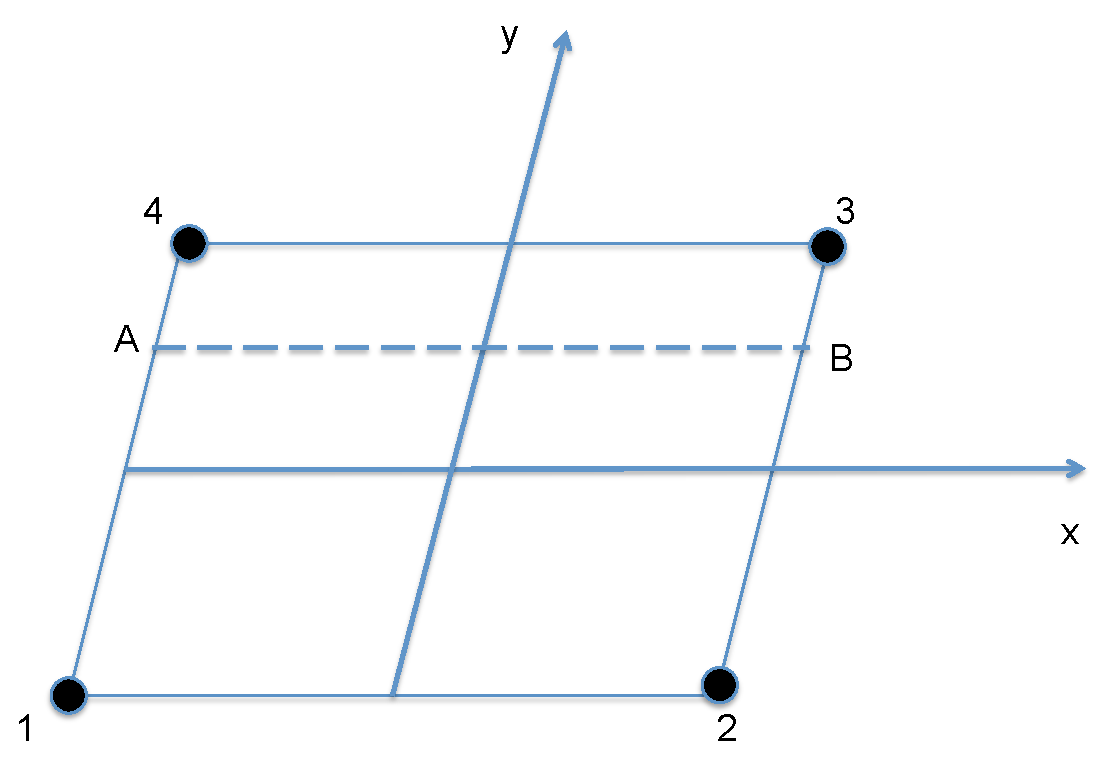
\includegraphics[width=10cm]{img/element.pdf}
\caption{Basic square domain}
\label{fig:element}
\end{figure}

We first fix $x = {x^A}$ and conduct 1-dimensional interpolation along the $y$ direction as discussed in the previous section as follows (see \cref{fig:onedimn});

\[f({x^A},y) = {L^1}(y){f^1} + {L^4}(y){f^4}\]

\begin{figure}[H]
\centering
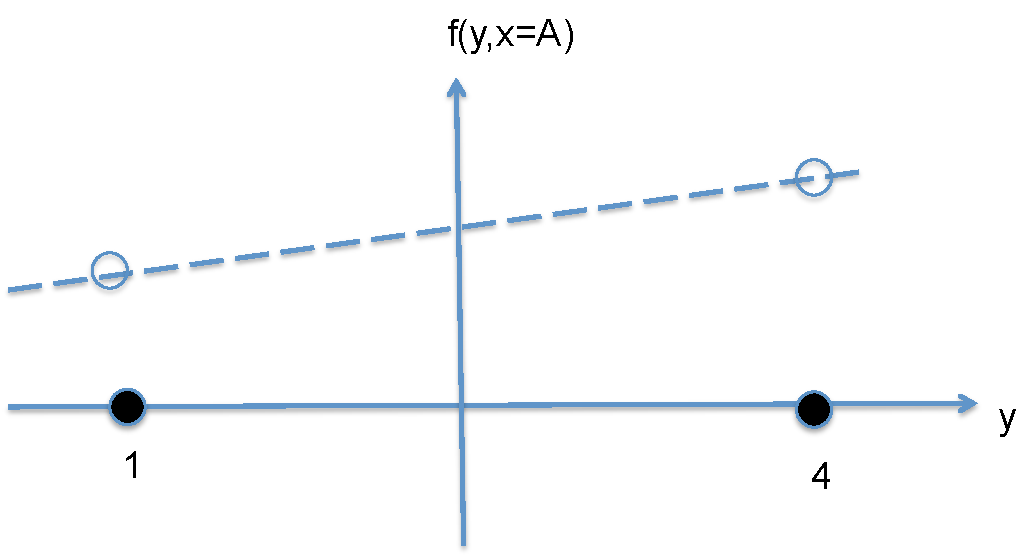
\includegraphics[width=10cm]{img/inter1D.pdf}
\caption{Interpolation along the $y$-direction}
\label{fig:onedimn}
\end{figure}

Similarly, we can fix $x = {x^B}$ and interpolate once again along the $y$ direction;

\[f({x^B},y) = {L^2}(y){f^2} + {L^3}(y){f^3}.\]

We now conduct the interpolation along the $x$-direction using the functions $f({x^A},y)$ and $f({x^B},y)$ respectively as follows;

\[f(x,y) = {L^A}(x){f({x^A},y)} + {L^B}(x){f({x^B},y)}.\]
\[f(x,y) = {L^A}(x)\left\{ {{L^1}(y){f^1} + {L^4}(y)f{}^4} \right\} + {L^B}(x)\left\{ {{L^2}(y){f^2} + {L^3}(y)f{}^3} \right\}\]
\[f(x,y) = {L^A}(x){L^1}(y){f^1} + {L^A}(x){L^4}(y)f{}^4 + {L^B}(x){L^2}(y){f^2} + {L^B}(x){L^3}(y)f{}^3\]


\begin{align*}
{L^A}(x) & \equiv {L^1}(\xi ) \\
{L^B}(x) & \equiv {L^2}(\xi ) \\
{L^1}(y) & \equiv {L^1}(\xi ) \\
{L^2}(y) & \equiv {L^1}(\xi ) \\
{L^3}(y) & \equiv {L^2}(\xi ) \\
{L^4}(y) & \equiv {L^2}(\xi )
\end{align*}

\[f(x,y) = {N^1}(x,y){f^1} + {N^2}(x,y){f^2} + {N^3}(x,y){f^3} + {N^4}(x,y){f^4}\]

\begin{align*}
{N^1}(x,y) & = {L^1}(x){L^1}(y) \\
{N^2}(x,y) & = {L^2}(x){L^1}(y) \\
{N^3}(x,y) & = {L^2}(x){L^2}(y) \\
{N^4}(x,y) & = {L^1}(x){L^2}(y)
\end{align*}


\subsection{Formulation of the finite element matrices}
We now discretize the principle of virtual work repeated below for completeness:

\begin{equation} \label{pvw_2}
\intL_V \sigma_{ij} \delta u_{i,j} dV - \intL_V f_i \delta u_i dV - \intL_{S_t} t_i^n \delta u_i dS = 0.
\end{equation}

For that purpose we will divide the complete domain $V$ into $N$-finite non-overlapping subdomains over each one of which we will approximate the solution in terms of local interpolating functions. Since the PVW (or weak form of the BVP) has been casted into an integral representation, it is possible to build the total integral considering the contribution of the $N$-sub-domains as follows;

\begin{equation}\label{pvw_dis}
\sum_{e=1}^{NEL} \intL_{V^e} \sigma_{ij} \delta u_{i,j} d{V^e} - \intL_V f_i \delta u_i d{V^e} - \intL_{S_t} t_i^n \delta u_id{S^e} = 0 
\end{equation}

For easiness consider a single subdomain
\begin{equation} \label{pvw_sing}
\intL_V \sigma_{ij} \delta u_{i,j} dV - \intL_V f_i\delta u_idV - \intL_{S_t} t_i^n \delta u_i dS = 0.
\end{equation}

The involved functions (e.g., displacements, strain, stresses) will be approximated via interpolation of the solution over a determined number of points termed in what follows nodes. Assume for instance that over element $e$ containing $n$ such nodes we know the displacements vector $u_i$. Furthermore, let the displacements for the $p$-node $u^P=[u^P, v^P, w^P]$. Using ideas from interpolation theory it is now possible to approximate the displacements vector over an arbitrary point $\vb{x}$ inside the element as follows
\[u_i(\vb x) = N_i^1(\vb x)u^1 + N_i^2(\vb x)u^2 + \cdots + N_i^P(\vb x)u^P + \cdots + N_i^n(\vb x)u^n\]
or in more general form
\begin{equation} \label{bas_interpol}
{u_i}(\vb x) = N_i^Q(\vb x){u^Q}
\end{equation}

and where the caption superscripts indicate summation over the number of nodes of the element while the subscript refers to the physical character of the variable being interpolated.

\begin{align*}
&\varepsilon_{ij}(\vb x) = B_{ij}^Q(\vb x){u^Q}\\
&\varepsilon_{ij}(\vb x) = \frac{1}{2}( u_{i,j} + u_{j,i} )\\
&\varepsilon_{ij}(\vb x) = \frac{1}{2}\left(\pdv{N_i^Q}{x_j} + \pdv{N_j^Q}{x_i} \right){u^Q}\\
&B_{ij}^Q = \frac{1}{2}\left(\pdv{N_i^Q}{x_j} + \pdv{N_j^Q}{x_i} \right)\\
&\delta {u_i} = N_i^Q(\vb x)\delta {u^Q}\\
&\intL_V C_{ijkl} B_{kl}^P u^P B_{ij}^Q\delta u^Q \dd{V} - \intL_V f_i N_i^Q\delta {u^Q}\dd{V}  - \intL_{S_t} t_i^n N_i^Q\delta {u^Q} \dd{S} = 0\\
&\delta {u^Q}\intL_V B_{ij}^Q C_{ijkl} B_{kl}^P\dd{V}{u^P} - \delta {u^Q}\intL_V N_i^Q{f_i}\dd{V}  - \delta {u^Q}\intL_{S_t} N_i^Qt_i^n\dd{S} = 0 \\
&\delta u^Q f_\sigma ^Q - \delta {u^Q}f_V^Q - \delta u^Q f_c^Q = 0\\
&f_\sigma ^Q - f_V^Q - f_c^Q = 0\\
&f_\sigma ^Q = \intL_V B_{ij}^Q C_{ijkl} B_{kl}^P\dd{V} u^P \equiv K^{QP} u^P\\
&f_V^Q = \intL_V N_i^Q f_i\dd{V} \\
&f_c^Q = \intL_{S_t} N_i^Qt_i^n \dd{S} \\
&K^{QP} u^P = f_V^Q + f_c^Q
\end{align*}

\subsubsection{Formulation in the physical space}
\subsubsection{Formulation in the natural space: the continuum mechanics analogy}
In typical finite element equilibrium equations we need to perform integration over the reference element domain $V_0(\vb{x})$ corresponding to originally arbitrarily shaped sub-domains as created during the meshing process.  In order to proceed with this integration it is useful to consider the following continuum mechanics analogy.

First assume that the actual physical domain $V_0(\vb{x})$ is the result of a deformation process imparted upon the natural domain as shown in \cref{fig:natural domain}. In this analogy, the physical domain $V_0(\vb{x})$ is regarded like a ``deformed'' configuration at an imaginary time $t=t$, while the natural ``undeformed'' domain $V(\vb{r})$   is treated like a reference undeformed configurations at time $t=0$. Both configurations are assumed to be connected through a deformation process;


\begin{equation}
\begin{aligned}
\vb{X}&=\vb{X}(\vb{r})\\
\vb{r}&=\vb{r}(\vb{X})
\end{aligned}
\label{eq:motion}
\end{equation}

\begin{figure}[h]
\centering
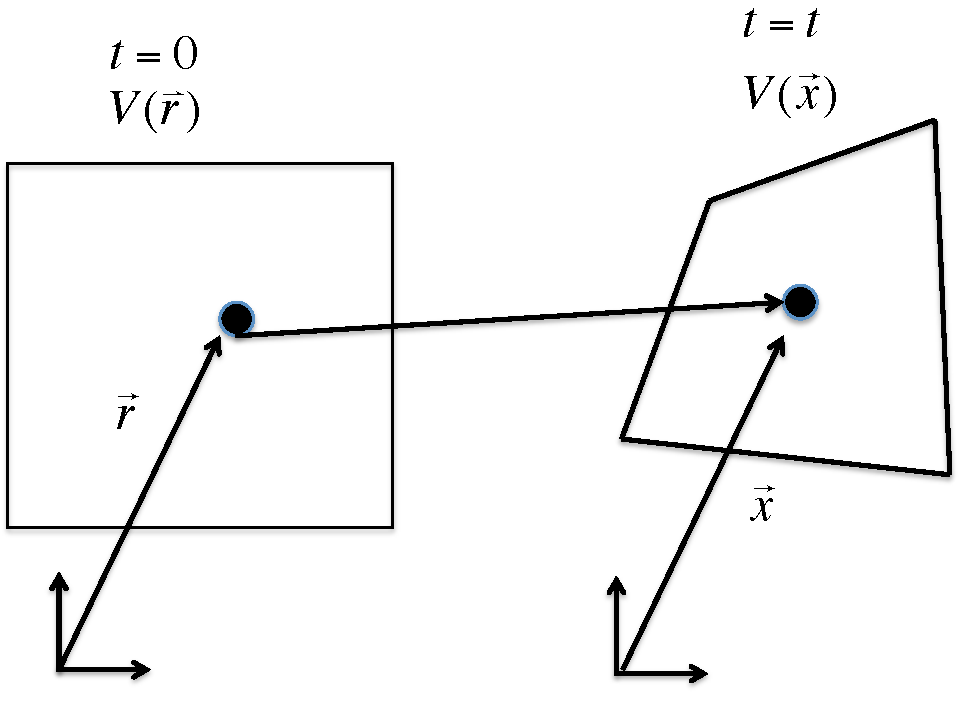
\includegraphics[width=8cm]{img/figure1.pdf}
\caption{Definition of the natural domain}
\label{fig:natural domain}
\end{figure}

 

In \cref{eq:motion} we can understand $\vb{r}$ like a material (Lagrangian) variable and $\vb{X}$ like a spatial (or Eulerian) variable. Using the continuum mechanics analogy it is clear that the ``deformation'' process at the continuum level is fully characterized by the ``deformation'' gradient or Jacobian of the transformation \cref{eq:motion} and defined according to;

\begin{equation}
dX_i=\dfrac{\partial X_i}{\partial r_J}dr_J\equiv J_{iJ}dr_{J}
\label{eq:gradient}
\end{equation}

where $dr_{J}$ and $dX_i$ represent material vectors in the original and deformed configuration. From \cref{eq:gradient} it is evident that the Jacobian contains all the information describing the change of the physical sub-domain with respect to the natural element. For the element integration process we will assume that every element $V(\vb{r})$ in the natural domain deforms into the physical element $V_0(\vb{X})$, thus allowing us to write typical terms like the ones in the material stiffness matrix
\begin{equation}
\intL_{V(\vb{X})} \hat{B}_{ij}^K(\vb{X}) C_{ijkl} \hat{B}_{kl}^P(\vb{X}) dV(\vb{X})\equiv \intL_{V_0(\vb{r})} \hat{B}_{ij}^K(\vb{r}) C_{ijkl} \hat{B}_{kl}^P(\vb{r})J dV_0(\vb{r})
\label{eq:matmatrix}
\end{equation}
where we have used $dV(\vb{X})=JdV(\vb{r})$, with $J$ being the determinant of the deformation gradient and in general we transform functions between the natural and physical space making use of \cref{eq:motion} according to
\begin{equation}
f(\vb{r})=F[\vb{X}(\vb{r})]
\label{eq:funtrans}
\end{equation}


\subsubsection*{Interpolation scheme}
Having identified the fact that the integration process will take place in the natural domain, we will approach the interpolation process directly in this natural space. In the case of the displacement based finite element method all the involved variables will then be obtained via interpolation of nodal displacements. For instance, assume that a given problem variable is defined in the physical space by the tensor $\Phi_{ik...p}(\vb{X})$. The interpolated variable is then written like;

\begin{equation}
\Phi_{ij...p}(\vb{X})=H_{ij...p}^K(\vb{r})\hat{u}^K
\label{eq:interpol}
\end{equation}

where $\hat{u}^K$ represents a vector of nodal points displacements, see \cref{fig:interpol nat dom}, and $H_{ij...p}^K(\vb{r})$ is an interpolator which keeps the tensorial character of the original physical variable $\Phi_{ik...p}(\vb{X})$ and where the super-index makes reference to a nodal identifier (with the summation convention in place).


\begin{figure}[h]
\centering
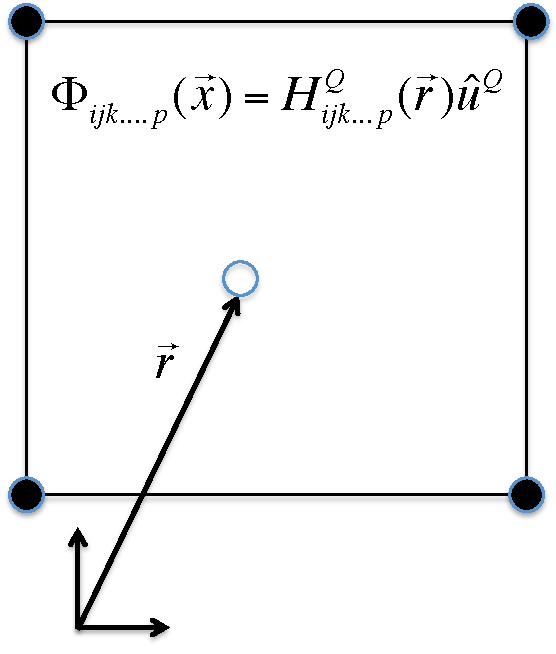
\includegraphics[width=4cm]{img/figure2.pdf}
\caption{General interpolation strategy in the natural domain}
\label{fig:interpol nat dom}
\end{figure}
 


Since the primary variable corresponds to displacements it must be kept in mind that $H_{ij...p}^K(\vb{r})$ corresponds to combinations of derivatives (or other arbitrary combinations) of the basic element shape functions defined in;


\begin{equation}
u_i(\vb{X})=N_i^K(\vb{r})\hat{u}^K
\label{eq:el interpol}
\end{equation}



For the general interpolation process we need two kinds of transformations.  First we need to transform integrals over the physical space into integrals into the natural space which corresponds to
\begin{equation}
\intL_{V(\vb{X})} F(\vb{X})dV(\vb{X})\equiv \intL_{V_0(\vb{r})} f(\vb{r})J dV_0(\vb{r})
\label{gen trans}
\end{equation}



Second we need to relate spatial differentiation in both, the physical and spatial domains.  Let us define these operators like $\nabla_i^X$ and $\nabla_I^r$ respectively. It then follows from \cref{eq:funtrans} that
\begin{equation}
\dfrac{\partial F}{\partial X_i}=\dfrac{\partial f}{\partial r_J}\dfrac{\partial r_J}{\partial X_i}
\label{eq:chain}
\end{equation}
from where we can establish the connection between the two operators like


\begin{equation}
\nabla_i^X=J_{iJ}^{-1}\nabla_J^r
\label{eq:fundamental}
\end{equation}


\subsubsection*{The fundamental interpolator}
We further define the fundamental interpolator giving rise to gradients of the primary displacement variable in the physical space according to
\begin{equation}
u_{i,j}(\vb{X})=L_{ij}^K(\vb{r})\hat{u}^K
\label{eq:fund operator}
\end{equation}


This fundamental interpolator  $L_{ik}^K(\vb{r})$ is derived after using \cref{eq:el interpol} and \cref{eq:fundamental} in the physical displacement gradient definition as shown next
\begin{align*}
u_{i,j}(\vb{X})&=\nabla_j^X u_i(\vb{X})\\
u_{i,j}(\vb{X})&=\nabla_j^X N_i^K(\vb{r})\hat{u}^K\\
u_{i,j}(\vb{X})&=J_{jQ}^{-1}\nabla_Q^r N_i^K(\vb{r})\hat{u}^K\\
u_{i,j}(\vb{X})&=J_{jQ}^{-1}N_{i,Q}^K(\vb{r})\hat{u}^K
\end{align*}
then
\begin{equation}
L_{ij}^K(\vb{r})=J_{jQ}^{-1}N_{i,Q}^K(\vb{r})
\label{eq:fundamental interpolator}
\end{equation}

\subsubsection*{Elemental stiffness matrix}
The elemental material stiffness matrix computed in the natural domain of \cref{fig:Nat domain} reads

\begin{equation}
K^{KP}=\intL_{V_0(\vb{r})} \hat{B}_{ij}^K(\vb{r}) C_{ijkl} \hat{B}_{kl}^P(\vb{r})J dV_0(\vb{r})\equiv \intL_{r=-1}^{r=+1}\intL_{s=-1}^{s=+1} \hat{B}_{ij}^K(r,s) C_{ijkl} \hat{B}_{kl}^P(r,s)J(r,s) \mathrm{d}r\mathrm{d}s
\label{eq:elematrix}
\end{equation}



\begin{figure}[h]
\centering
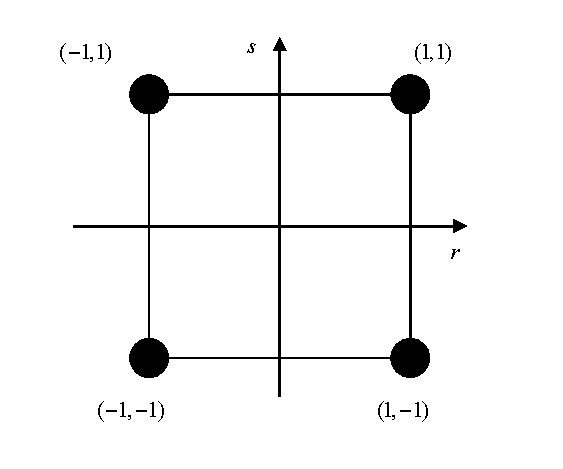
\includegraphics[width=6cm]{img/figure3.pdf}
\caption{Natural domain of integration}
\label{fig:Nat domain}
\end{figure}
 

Once the interpolator $\hat{B}_{ij}^K(\vb{r})$ has been identified the elemental stiffness matrix is obtained via numerical integration (quadrature) as described in \eqref{eq:eleintegration}

\begin{equation}
\intL_{r=-1}^{r=+1}\intL_{s=-1}^{s=+1} \hat{B}_{ij}^K(r,s) C_{ijkl} \hat{B}_{kl}^P(r,s)J(r,s) \mathrm{d}r\mathrm{d}s\approx \sum_{i,j=1}^\text{NGPTS} \alpha_i \alpha_j \hat{B}_{kl}^K(r_i,s_j)C_{ijkl} \hat{B}_{kl}^P(r_i,s_j) J(r_i,s_j)
\label{eq:eleintegration}
\end{equation}


and where NGPTS corresponds to the number of integration points, $\alpha_j$ is a weighting factor and $r_i,s_j$   are the coordinates of a typical point $\vb{r}$ in the natural space of \cref{fig:Nat domain}.

 
\begin{figure}[h]
\centering
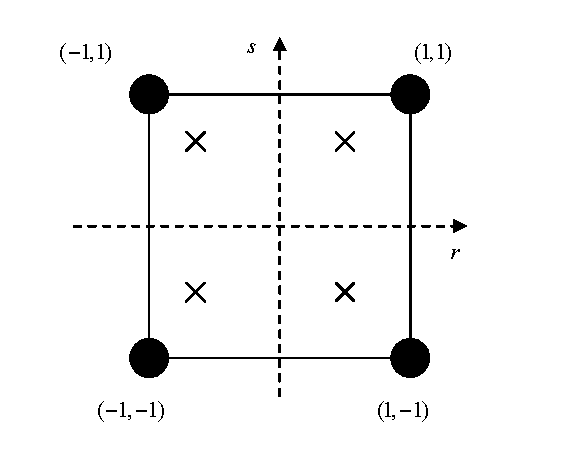
\includegraphics[width=6cm]{img/figure4.pdf}
\caption{Natural integration domain showing quadrature evaluation nodes}
\label{fig:integration domain}
\end{figure}	 


One important aspect of the numerical integration that has to be kept in mind is accuracy.  Depending on the particularly selected integration scheme, the number of introduced integration points fixes the maximum polynomial order of the considered functions that can be integrated accurately.  In the case of the integrand in \cref{eq:eleintegration}, it is clear that this order increases as the distortion of the physical element  with respect to the natural element increases.  One way of dealing with this dependency of accuracy with element distortion is to make use of adaptative integration techniques which are numerically expensive.  What is actually done in standard FEM analysis is to choose the number of quadrature points beforehand and introduce distortion related error criteria inside the code in such a way that some sort of validation is performed before the numerical integration process is started.

\subsubsection*{Strain displacement interpolator for the infinitesimal strain tensor}
The $Q$-th nodal contribution to the infinitesimal strain-displacement interpolator can be obtained in explicit form as follows. Let $L_x^Q$ and $L_y^Q$ be the spatial differential operators in $x$ and $y$ respectively. We have after expanding \cref{eq:fundamental interpolator}
%
\begin{align*}
L_x^Q & = J_{xP}^{-1}\frac{\partial N^Q}{\partial r_P} \equiv J_{xr}^{-1}\frac{\partial N^Q}{\partial r} + J_{xs}^{-1}\frac{\partial N^Q}{\partial s}\\
L_y^Q & = J_{yP}^{-1}\frac{\partial N^Q}{\partial r_P} \equiv J_{yr}^{-1}\frac{\partial N^Q}{\partial r} + J_{ys}^{-1}\frac{\partial N^Q}{\partial s}
\end{align*}
%
or in matrix form
%
\begin{equation}
\begin{Bmatrix}
L_x^Q\\
L_y^Q
\end{Bmatrix} = 
\begin{bmatrix}
J_{xP}^{-1} &J_{xs}^{- 1}\\
J_{yr}^{-1} &J_{ys}^{- 1}
\end{bmatrix}
\begin{Bmatrix}
\frac{\partial N^Q}{\partial r}\\
\frac{\partial N^Q}{\partial s}
\end{Bmatrix}
\end{equation}

The $Q$-th nodal contribution is then assembled as follows;


\begin{equation}
\begin{Bmatrix}
\pdv{u}{x}\\
\pdv{v}{y}\\
\pdv{u}{y} + \pdv{v}{x}
\end{Bmatrix} =
\begin{bmatrix}
 &L_x^Q &0 \\
\cdots &0 &L_y^Q &\cdots\\
 &L_y^Q &L_{xy}^Q
\end{bmatrix}
\begin{Bmatrix}
\vdots\\
u^Q\\
v^Q\\
\vdots
\end{Bmatrix}
\label{eq:strain inter}
\end{equation}

\begin{algorithm}[H]
\SetAlgoLined
\KwData{Nodal coordinates $x^Q$}
\KwResult{Strain-displacement interpolator $B_{ij}^Q$ }
Compute Jacobian ${J_{iJ}} = \pdv{N_i^Q}{r_J}{\hat x}^Q$\\
Invert Jacobian  ${J_{iJ}} \to J_{iJ}^{ - 1}$\\
Compute fundamental interpolator $L_{ij}^Q = J_{jP}^{ - 1}\pdv{N_i^Q}{r_P}$\\
Assemble $B_{ij}^Q = \frac{1}{2}\left( {L_{ij}^Q + L_{ji}^Q} \right)$ 
\caption{Strain-displacement interpolator}
\end{algorithm}


